\documentclass{article}
\usepackage[utf8]{inputenc}
\usepackage[legalpaper, margin=1in]{geometry}

\usepackage[english]{babel}

\usepackage{amsmath}
\usepackage{amssymb}
\usepackage{amsthm}
\usepackage{physics}

\usepackage{graphicx}
\usepackage{booktabs}

\usepackage{xcolor}
\usepackage{listings}
\usepackage{makecell}

\usepackage{hyperref}
\usepackage{cleveref}

\usepackage{marginnote}
\usepackage{csquotes}
\usepackage{todonotes}

\usepackage{listings}
\usepackage{xcolor}
\definecolor{codegreen}{rgb}{0,0.6,0}
\definecolor{codegray}{rgb}{0.5,0.5,0.5}
\definecolor{codepurple}{rgb}{0.58,0,0.82}
\definecolor{backcolour}{rgb}{0.95,0.95,0.92}
\lstdefinestyle{mystyle}{
    backgroundcolor=\color{backcolour},   
    commentstyle=\color{codegreen},
    keywordstyle=\color{magenta},
    numberstyle=\tiny\color{codegray},
    stringstyle=\color{codepurple},
    basicstyle=\ttfamily\footnotesize,
    breakatwhitespace=false,         
    breaklines=true,                 
    captionpos=b,                    
    keepspaces=true,                 
    numbers=left,                    
    numbersep=5pt,                  
    showspaces=false,                
    showstringspaces=false,
    showtabs=false,                  
    tabsize=2
}
\lstset{style=mystyle}

\newtheorem{definition}{Definition}
\newtheorem{theorem}{Theorem}
\newtheorem{lemma}{Lemma}
\newtheorem{corollary}[lemma]{Corollary}
\newtheorem{property}{Property}

% Start every section on new page
% \usepackage{titlesec}
% \newcommand{\sectionbreak}{\clearpage}

%\usepackage[xcolor,leftbars]{changebar}
%\usepackage{color}
% \cbcolor{red}
%\newenvironment{question}%
%{\begin{quote}%
%  \begin{changebar}\cbcolor{gray}\color{black}}%
%  {\end{changebar}%
%\end{quote}}

%\usepackage[svgnames]{xcolor}
%\usepackage{framed}
%\definecolor{shadecolor}{named}{LightGray}

\title{CSC2516: Programming Assignment 3: Attention-Based Neural Machine Translation}
\author{}
\date{March 2021}

\begin{document}

\maketitle

\section*{Part 1: LSTMs}

\subsection*{1. LSTM Training}

\begin{quote}
A screenshot of your \texttt{fullMyLSTMCell} implementation
\end{quote}

\begin{lstlisting}[language=Python]
class MyLSTMCell(nn.Module):
    def __init__(self, input_size, hidden_size):
        super(MyLSTMCell, self).__init__()

        self.input_size = input_size
        self.hidden_size = hidden_size

        # ------------
        # FILL THIS IN
        # ------------
        self.Wii = nn.Linear(input_size, hidden_size)
        self.Whi = nn.Linear(hidden_size, hidden_size)

        self.Wif = nn.Linear(input_size, hidden_size)
        self.Whf = nn.Linear(hidden_size, hidden_size)

        self.Wig = nn.Linear(input_size, hidden_size)
        self.Whg = nn.Linear(hidden_size, hidden_size)

        self.Wio = nn.Linear(input_size, hidden_size)
        self.Who = nn.Linear(hidden_size, hidden_size)


    def forward(self, x, h_prev, c_prev):
        """Forward pass of the LSTM computation for one time step.

        Arguments
            x: batch_size x input_size
            h_prev: batch_size x hidden_size
            c_prev: batch_size x hidden_size

        Returns:
            h_new: batch_size x hidden_size
            c_new: batch_size x hidden_size
        """

        # ------------
        # FILL THIS IN
        # ------------
        i = torch.sigmoid(self.Wii(x) + 
                          self.Whi(h_prev))
        f = torch.sigmoid(self.Wif(x) + 
                          self.Whf(h_prev))
        g = torch.tanh(self.Wig(x) + 
                       self.Whg(h_prev))
        o = torch.sigmoid(self.Wio(x) + 
                          self.Who(h_prev))
        c_new = f * c_prev + i * g
        h_new = o * torch.tanh(c_new)
        return h_new, c_new
\end{lstlisting}


\begin{quote}
... the loss plots output by \texttt{save\_loss\_comparison\_lstm}
\end{quote}

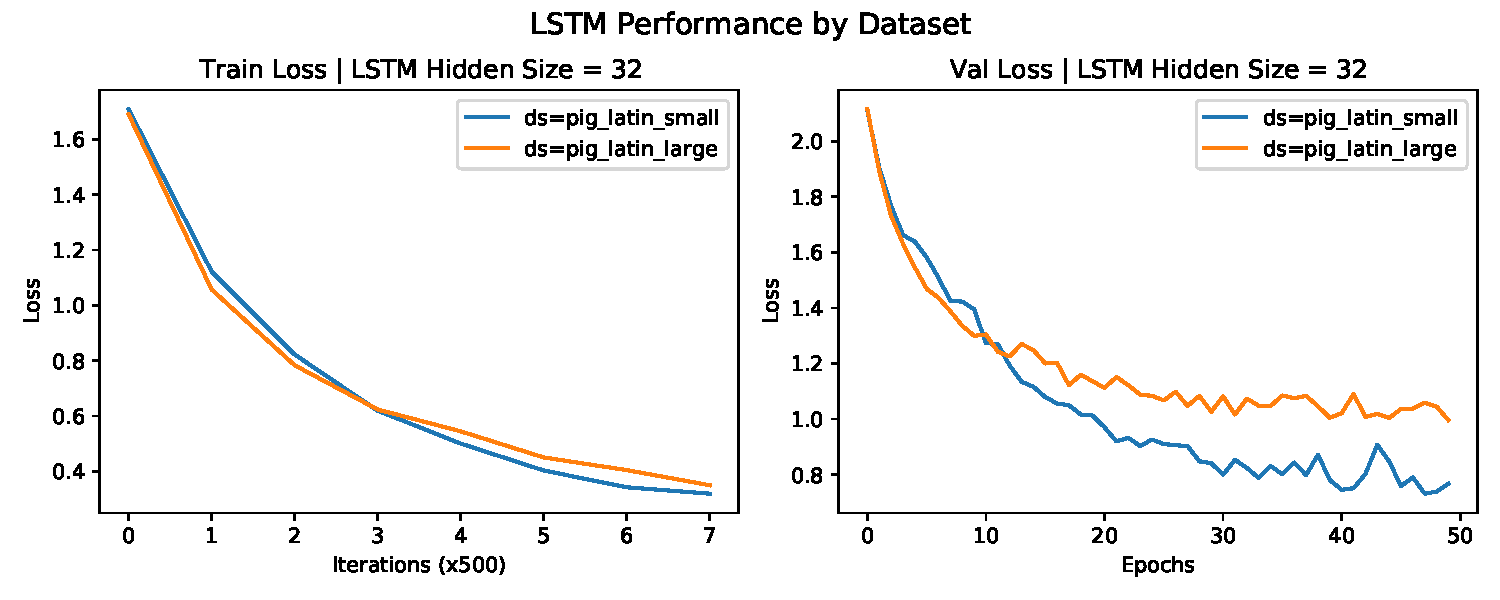
\includegraphics[width=\linewidth]{loss_plot_lstm}

\begin{quote}
... and your analysis

Does  either  model perform significantly better?  Why might this be the case?
\end{quote}

While the training loss were similar, the \texttt{pig\_latin\_small} model (blue) performed better with lower validation loss than \texttt{pig\_latin\_large} (orange). The small model was trained with smaller batch sizes (\texttt{'batch\_size':64}), which contributed to better generalization ability than ones trained with larger batch sizes (\texttt{'batch\_size':512}). [Reference: Keskar NS, Mudigere D, Nocedal J, Smelyanskiy M, Tang PT. On large-batch training for deep learning: Generalization gap and sharp minima. arXiv preprint arXiv:1609.04836. 2016 Sep 15.]



\subsection*{2 Model Failure}

\begin{quote}
Identify a distinct failure mode and briefly describe it.
\end{quote}
Example below:

\begin{lstlisting}
source:		bond-street print-shops are good-for-nothing 
translated:	ondertay-inbay inptray-ospatshay areway oodgay-orfay-othingn

ground-truth: ondbay-eetstray intpray-opsshay areway oodgay-orfay-othingnay
\end{lstlisting}

It appears that the model fails at edge-case words with hyphens. % and often fails at words that start with vowel, with which it often correctly adds ``-ay'' at the end but scrambles the other letters.


\subsection*{3 Model size}


\begin{quote}
Write down the number of LSTM units and number of connections in this encoder model as a function of H, K, and D.
\end{quote}

Number of LSTM units: $1$. (One unique \texttt{MyLSTMCell} is shared across all encoder time steps)

Calculation for number of connections: 

For each LSTM time step, ignoring activation functions:

%\begin{itemize}
%\item 
%Within each LSTM time step, ignoring activation functions (total $(4(DH+HH)+6H)$): 
\begin{itemize}
\item 
$4(DH+HH)$ for computing $i$, $f$, $g$, $o$
\item
$4H$ for computing $c$ with two element-wise multiplications involving total of four input vectors
\item
$2H$ for computing $h$ with one element-wise multiplication involving two input vectors
\end{itemize}

Finally, the last step of the encoder has an out put connection of $H$ for $h^{enc}_T$. Therefore, in total for $K$ time steps, there are: $K(4(DH+HH)+6H)+H$ connections.

%\end{itemize}

% $(H+H+D) \times K + H+H$. (Each of the $K$ units receives the previous hidden state (\texttt{h\_prev}) and the previous cell state (\texttt{c\_prev}) input with $H+H$ connections and the current word's embedding input with $D$ connections, and the encoder final hidden and cell state output with $H+H$ dimensions)


\pagebreak
\section*{Part 2: Additive Attention}

\subsection*{1}

\begin{quote}
Write  down  the  mathematical  expression  for  these  quantity
\end{quote}

\begin{align*}
\tilde{\alpha}^{(t)}_i &= W_2^\intercal \textrm{ReLU} ( W_1^\intercal 
\begin{bmatrix}
Q_t \\ K_i
\end{bmatrix} 
)
\\
\alpha^{(t)}_i &= \textrm{softmax}(\tilde{\alpha}^{(t)})_i = \frac
{\exp(\tilde{\alpha}^{(t)}_i)}
{\sum_{j=1}^{\textrm{seq\_len}} \exp(\tilde{\alpha}^{(t)}_j) }
\\
c_t &= {\alpha^{(t)}}^\intercal K = \sum_{i=1}^{\textrm{seq\_len}} \alpha^{(t)}_i K_i
\end{align*}

\subsection*{2}

\begin{quote}
Training/validation plots 
\end{quote}

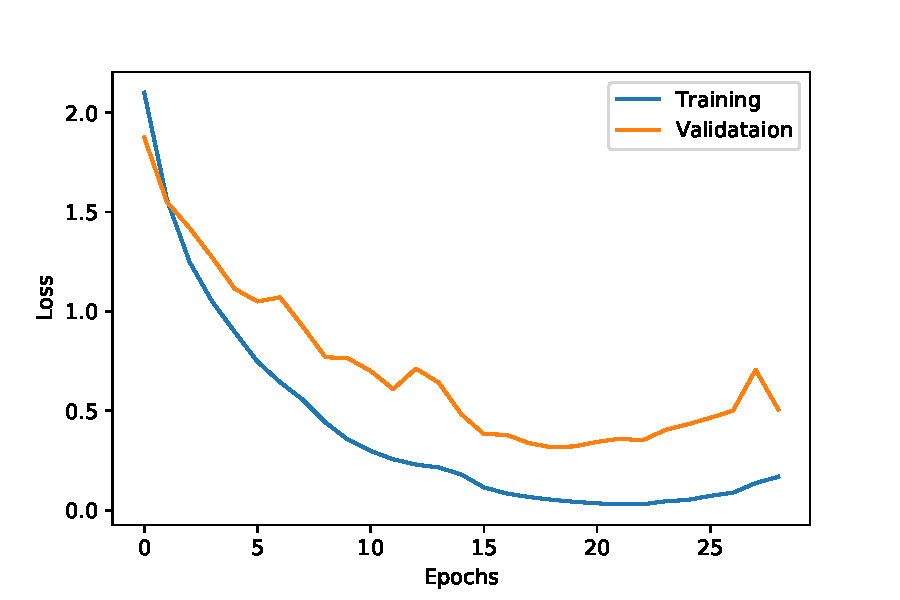
\includegraphics[width=\linewidth]{loss_additive_attention}

\begin{quote}
Find  one training example where the decoder with attention performs better than the decoder without attention.
\end{quote}

Pass [0 pt].
 
\subsection*{3}

\begin{quote}
How does the training speed compare?  Why?
\end{quote}

The training speed is faster with the attention model which reached less than $1.0$ validation loss within 7 epochs, whereas previously it took the ``small'' non-attention model 20 epochs to reach this level of validation loss. Attention model can train faster because the current word-for-word translation task can be much more efficiently accomplished if the decoder can learn to selectively ``attend'' to only the word at the current position.

\subsection*{4}

\begin{quote}
 number of LSTM units in \texttt{RNNAttentionDecoder}:
\end{quote}

$1$ unique LSTM unit shared across all time steps of the decoder.

\begin{quote}
the number of connections in the above computation:
\end{quote}

For each of the $K$ decode time steps, the decoder has:

\begin{itemize}
\item 
Attention computation for each time step: $K(2H\times H+H\times 1)$ for the fully connected attention network and $KH$ to compute the weighted context vector (ignoring softmax computation)

\item 
Connections in each LSTM time step is $4(DH+HH)$ as discussed in Part 1.3. 

\item
Output connections from each decoder LSTM unit: $H\times V$ for the linear layer from hidden state to output vocabulary

\end{itemize}


Total number of connections in decoder network: $K[K(2HH+H)+4(DH+HH)+(HV)]$



\pagebreak
\section*{Part 3: Scaled Dot Product Attention}

\subsection*{1}

\begin{lstlisting}[language=Python]
class ScaledDotAttention(nn.Module):

	...

    def forward(self, queries, keys, values):

    	...

        # ------------
        # FILL THIS IN
        # ------------
        batch_size, k, hidden_size = queries.shape
        batch_size, seq_len, hidden_size = keys.shape
        # q = 
        # k = 
        # v = 
        unnormalized_attention = (self.Q(queries) @ 
                                  self.K(keys).transpose(2,1) * 
                                  self.scaling_factor)
        # assert unnormalized_attention.shape == (batch_size, k, seq_len)
        # Softmax over seq_len and dim = 1
        attention_weights = self.softmax(unnormalized_attention.transpose(2,1))
        # assert attention_weights.shape == (batch_size, seq_len, k)
        context = context = attention_weights.transpose(2, 1) @ self.V(values)
        # assert context.shape == (batch_size, k, hidden_size)
        return context, attention_weights


\end{lstlisting}


\subsection*{2}

\begin{lstlisting}[language=Python]
        
class CausalScaledDotAttention(nn.Module):
    def __init__(self, hidden_size):
        ...
    
    def forward(self, queries, keys, values):
        ...

        # ------------
        # FILL THIS IN
        # ------------

        batch_size, k, hidden_size = queries.shape
        batch_size, seq_len, hidden_size = keys.shape
        # q = 
        # k = 
        # v = 
        unnormalized_attention = (self.Q(queries) @ 
                                  self.K(keys).transpose(2,1) * 
                                  self.scaling_factor)
        # Causal mask
        mask = torch.triu(torch.full_like(unnormalized_attention, 
                                          fill_value=self.neg_inf), 
                          diagonal=+1)
        unnormalized_attention += mask
        # assert unnormalized_attention.shape == (batch_size, k, seq_len)
        # Softmax over seq_len and dim = 1
        attention_weights = self.softmax(unnormalized_attention.transpose(2,1))
        # assert attention_weights.shape == (batch_size, seq_len, k)
        context = attention_weights.transpose(2, 1) @ self.V(values)
        # assert context.shape == (batch_size, k, hidden_size)
        return context, attention_weights
\end{lstlisting}

\subsection*{3}

\begin{quote}
For this question, describe why we need to represent the position of each word through this positional encoding in one or two sentences.  Additionally, describe the advantages of using this positional encoding method, as opposed to other positional encoding methods such as a one hot encoding in one or two sentences.
\end{quote}

Positional encoding is used to add temporal information about at which position the word came from, in addition to embedding of the word. The sinusoidal positional embedding uses unique sinusoidal values with the same dimension as the hidden layer such that the word embedding and positional embedding can be easily summed independent of the sequence length; with one-hot encoding, the positional encoding has to be at least the same dimension as the longest sequence and cannot be efficiently combined with the hidden states.



\subsection*{4}

\begin{quote}
How do the translation results compare to the previous decoders?
\end{quote}

The transformer model performed well on simple words but similar to previous decoders struggled with longer words like ``conditioning''.

\subsection*{5}

\begin{quote}
Run these experiments,  and report the effects of increasing model capacity via the hiddensize, and the effects of increasing dataset size
\end{quote}

\includegraphics[width=\linewidth]{loss_plot_trans_by_dataset}

\includegraphics[width=\linewidth]{loss_plot_trans_by_hidden}

\begin{lstlisting}[language=Python]
================================================================================
                                      Opts                                      
--------------------------------------------------------------------------------
                         data_file_name: pig_latin_small                        
                                   cuda: 1                                      
                                nepochs: 100                                    
                         checkpoint_dir: checkpoints                            
                          learning_rate: 0.0005                                 
                early_stopping_patience: 100                                    
                               lr_decay: 0.99                                   
                             batch_size: 64                                     
                            hidden_size: 32                                     
                           encoder_type: transformer                            
                           decoder_type: transformer                            
                 num_transformer_layers: 3                                      
================================================================================
...
Epoch:  99 | Train loss: 0.082 | Val loss: 0.930 | Gen: ethay arrway onditiongcatinay isway orkingway
Obtained lowest validation loss of: 0.837032363191247
source:		the air conditioning is working 
translated:	ethay arrway onditiongcatinay isway orkingway



================================================================================
                                      Opts                                      
--------------------------------------------------------------------------------
                         data_file_name: pig_latin_large                        
                                   cuda: 1                                      
                                nepochs: 100                                    
                         checkpoint_dir: checkpoints                            
                          learning_rate: 0.0005                                 
                early_stopping_patience: 10                                     
                               lr_decay: 0.99                                   
                             batch_size: 512                                    
                            hidden_size: 32                                     
                           encoder_type: transformer                            
                           decoder_type: transformer                            
                 num_transformer_layers: 3                                      
================================================================================
...
Epoch:  99 | Train loss: 0.090 | Val loss: 0.439 | Gen: ethay iriway onditiongcay isway orkingway
Obtained lowest validation loss of: 0.43923975067775484
source:		the air conditioning is working 
translated:	ethay iriway onditiongcay isway orkingway


================================================================================
                                      Opts                                      
--------------------------------------------------------------------------------
                         data_file_name: pig_latin_small                        
                                   cuda: 1                                      
                                nepochs: 50                                     
                         checkpoint_dir: checkpoints                            
                          learning_rate: 0.0005                                 
                early_stopping_patience: 20                                     
                               lr_decay: 0.99                                   
                             batch_size: 64                                     
                            hidden_size: 64                                     
                           encoder_type: transformer                            
                           decoder_type: transformer                            
                 num_transformer_layers: 3                                      
================================================================================
...
Epoch:  49 | Train loss: 0.006 | Val loss: 0.493 | Gen: ethay airway onditioningcay isway orkingway
Obtained lowest validation loss of: 0.41776718463079304
source:		the air conditioning is working 
translated:	ethay airway onditioningcay isway orkingway


================================================================================
                                      Opts                                      
--------------------------------------------------------------------------------
                         data_file_name: pig_latin_large                        
                                   cuda: 1                                      
                                nepochs: 50                                     
                         checkpoint_dir: checkpoints                            
                          learning_rate: 0.0005                                 
                early_stopping_patience: 20                                     
                               lr_decay: 0.99                                   
                             batch_size: 512                                    
                            hidden_size: 64                                     
                           encoder_type: transformer                            
                           decoder_type: transformer                            
                 num_transformer_layers: 3                                      
================================================================================
...
Epoch:  49 | Train loss: 0.044 | Val loss: 0.459 | Gen: ethay airway ondidioningcay isway orkingway
Obtained lowest validation loss of: 0.45930340046607804
source:		the air conditioning is working 
translated:	ethay airway ondidioningcay isway orkingway
\end{lstlisting}

The larger model with larger hidden size was able to reduce the validation loss on the small data set but might had over-fitted given the small training loss of 0.006. The larger model did not have an effect on the large data size's loss statistics. The translation quality was in general better with the larger models, which were able to correctly translate ``air'' and the small dataset model was able to correct translate challenging long words like `conditioning''.

\subsection*{6} 

Pass [0 pt]

\subsection*{7}

The additive attention model concatenates the Query and Key vectors thus treating all dimensions as independent feature inputs to the fully connected model, and allows non-linear relationships to be expressed using ReLU. There are more parameters involved which make it more expressive at the potentially cost of training difficulty and over-fitting. 

In contrast, the dot product model preserves the dimensional correspondence between the Query and Key vectors by applying separate linear mappings and then calculating the dot product. All operations are linear which limits its expressiveness but the dot product model has a more intuitive interpretation and less parameters to train.


\pagebreak
\section*{Part 4: Fine-tuning for arithmetic sentiment analysis}

\subsection*{1}

\begin{quote}
add a classifier for the GPT model
\end{quote}

Adding a two-layer MLP:

\begin{lstlisting}[language=Python]
from transformers import OpenAIGPTForSequenceClassification
class GPTCSC413(OpenAIGPTForSequenceClassification):
    def __init__(self, config):
        super(GPTCSC413, self).__init__(config)
        # Your own classifier goes here
        # score is name for the classifier in OpenAIGPTForSequenceClassification, similar as the self.classifier in BertForSequenceClassification
        self.score = nn.Sequential(
            nn.Linear(config.hidden_size, config.hidden_size),
            nn.ReLU(),
            nn.Linear(config.hidden_size, self.config.num_labels)
            )


\end{lstlisting}


\subsection*{2 BERT frozen vs finetune}

The finetune model performed much better than the frozen model on validation --- the frozen model barely improved the validation accuracy during training and simply predicted all expressions to be positive during testing. Both models failed completely on neural expressions, which may be due to lack of training examples and the difficulty to precisely predict neutrality.

Frozen BERT training curve:

\includegraphics[width=\linewidth]{part4_bert_freeze}

\begin{lstlisting}[language=Python]
======== Epoch 4 / 4 ========
Training...

  Average training loss: 0.70
  Training epcoh took: 0:00:10
Running Validation...
  Accuracy: 0.74
  Validation took: 0:00:02

Training complete!

Predicting labels for 160 test sentences...
Number of expressions with negative result 47 
 0  predicted correctly , accuracy  0.0 

Number of expressions with 0 result 2 
 0  predicted correctly , accuracy  0.0 

Number of expressions with positive result 111 
 111  predicted correctly , accuracy  1.0 

\end{lstlisting}

Finetune BERT training curve:

\includegraphics[width=\linewidth]{part4_bert_finetune}

\begin{lstlisting}[language=Python]
======== Epoch 4 / 4 ========
Training...

  Average training loss: 0.28
  Training epcoh took: 0:00:42
Running Validation...
  Accuracy: 0.95
  Validation took: 0:00:02

Training complete!



Predicting labels for 160 test sentences...
Number of expressions with negative result 47 
 47  predicted correctly , accuracy  1.0 

Number of expressions with 0 result 2 
 0  predicted correctly , accuracy  0.0 

Number of expressions with positive result 111 
 109  predicted correctly , accuracy  0.9819819819819819 

\end{lstlisting}



\subsection*{3 BERT vs GPT}

The GPT model performed almost identically to the BERT model in overall testing. However, in the select test cases below, GPT was able to correctly classify ``one minus zero'' as positive where as BERT failed to do so.

Finetune GPT training:

\includegraphics[width=\linewidth]{part4_gpt_finetune}

\begin{lstlisting}[language=Python]
======== Epoch 4 / 4 ========
Training...

  Average training loss: 0.22
  Training epcoh took: 0:00:47
Running Validation...
  Accuracy: 0.95
  Validation took: 0:00:03

Training complete!


Predicting labels for 160 test sentences...
Number of expressions with negative result 47 
 47  predicted correctly , accuracy  1.0 

Number of expressions with 0 result 2 
 0  predicted correctly , accuracy  0.0 

Number of expressions with positive result 111 
 108  predicted correctly , accuracy  0.972972972972973 

\end{lstlisting}


Comparison of interesting test cases: In the examples above, we test the model for ``one minus X'' and ``X minus one''. It seems that the BERT model simply learned that, since ``one'' is a small number, if a sentence starts with ``one minus'' the result would be negative. Also interestingly both models classified ``one minus one'' to be negative. 


\begin{lstlisting}[language=Python]
Test input: one minus zero
    model_finetune_bert: negative
    model_finetune_gpt: positive
Test input: one minus one
    model_finetune_bert: negative
    model_finetune_gpt: negative
Test input: one minus two
    model_finetune_bert: negative
    model_finetune_gpt: negative
Test input: one minus three
    model_finetune_bert: negative
    model_finetune_gpt: negative
Test input: one minus four
    model_finetune_bert: negative
    model_finetune_gpt: negative
Test input: one minus five
    model_finetune_bert: negative
    model_finetune_gpt: negative
Test input: zero minus one
    model_finetune_bert: negative
    model_finetune_gpt: negative
Test input: one minus one
    model_finetune_bert: negative
    model_finetune_gpt: negative
Test input: two minus one
    model_finetune_bert: negative
    model_finetune_gpt: negative
Test input: three minus one
    model_finetune_bert: positive
    model_finetune_gpt: positive
Test input: four minus one
    model_finetune_bert: positive
    model_finetune_gpt: positive
Test input: five minus one
    model_finetune_bert: positive
    model_finetune_gpt: positive

\end{lstlisting}

\subsection*{4 BERT vs GPT application}

GPT is better suited for text sequence prediction tasks because it is trained with an auto-regressive model and processes text unidirectionally.

\subsection*{5 Exploration}

Pass [0 pt]


\end{document}
